\documentclass[a4paper,12pt]{article}

% Основные пакеты
\usepackage[T1, T2A]{fontenc}
\usepackage[utf8]{inputenc}
\usepackage[english, russian]{babel}
\usepackage{geometry}
\usepackage{indentfirst}
\usepackage{graphicx}
\usepackage{wrapfig}
\usepackage{amsmath, amssymb, amsfonts}
\usepackage{braket} 
\usepackage{float}
\usepackage{amsmath}  % для математических окружений
\usepackage{bm}  
% Гиперссылки и цветовые настройки
\usepackage[dvipsnames]{xcolor}
\usepackage[colorlinks]{hyperref}
\hypersetup{
	linkcolor=blue,
	filecolor=magenta,
	urlcolor=cyan
}

\usepackage{listings}
\usepackage{xcolor}

% Цвета
\definecolor{backcolour}{rgb}{0.95,0.95,0.92}
\definecolor{codegreen}{rgb}{0, 0.5, 0}
\definecolor{codegray}{rgb}{0.4, 0.4, 0.4}
\definecolor{codepurple}{rgb}{0.58, 0, 0.82}
\definecolor{keywordcolor}{rgb}{0.0, 0.2, 0.7}
\definecolor{stringcolor}{rgb}{0.6, 0, 0}
\definecolor{framecolor}{rgb}{0.7, 0.7, 0.7}

% Стиль для Mathematica
\lstdefinestyle{python}{
	language=python,
	backgroundcolor=\color{backcolour},
	basicstyle=\ttfamily\small,
	keywordstyle=\color{keywordcolor}\bfseries,
	commentstyle=\color{codegreen}\itshape,
	stringstyle=\color{stringcolor},
	numberstyle=\tiny\color{codegray},
	numbers=left,
	numbersep=5pt,
	breaklines=true,
	breakatwhitespace=false,
	showstringspaces=false,
	keepspaces=true,
	frame=single,
	rulecolor=\color{framecolor},
	frameround=tttt,
	captionpos=b,
	tabsize=2,
	xleftmargin=1em,
	xrightmargin=0.5em
}

% Установить стиль по умолчанию
\lstset{style=python}

% Путь к изображениям
\graphicspath{{./images/}}

% Геометрия страницы
\geometry{left=2cm, right=2cm, bottom=2cm, top=2cm}

\begin{document}
	\begin{titlepage}
		\centering
		\vspace*{1cm}
		
		{\large Министерство науки и высшего образования Российской Федерации}\\
		{\large ФЕДЕРАЛЬНОЕ ГОСУДАРСТВЕННОЕ АВТОНОМНОЕ ОБРАЗОВАТЕЛЬНОЕ УЧРЕЖДЕНИЕ ВЫСШЕГО ОБРАЗОВАНИЯ «НАЦИОНАЛЬНЫЙ ИССЛЕДОВАТЕЛЬСКИЙ УНИВЕРСИТЕТ ИТМО»}\\
		{\large (УНИВЕРСИТЕТ ИТМО)}\\
		
		\vspace{2cm}
		
		{\large Факультет «Систем управления и робототехники»}\\
		
		\vspace{3cm}
		
		\textbf{{\Huge ОТЧЕТ}\\
			{\Huge О ЛАБОРАТОРНОЙ РАБОТЕ №6}}\\
		
		\vspace{1cm}
		
		{\LARGE По дисциплине «Частотные методы»}\\
		{\LARGE на тему: «Обработка изображений»}\\
		
		\vspace{3cm}
		
		{\Large Студент:}\\
		Охрименко Ева
		
		\vspace{2cm}
		
		{\Large Преподаватели:}\\
		Догадин Егор Витальевич\\
		Пашенко Артем Витальевич\\
		
		\vspace{3cm}
		{\large г. Санкт-Петербург}\\
		{\large 2025}
		
	\end{titlepage}
	\newpage
	\tableofcontents
	\newpage
	
\section{Задание.  Фильтрация изображений с периодичностью.}

В этом задании мне нужно сделать фильтрацию периодических шумов на изображении с использованием двумерного преобразования Фурье.\\	

\textbf{Ожидаемые результаты}
\begin{itemize}
	\item Исходное изображение
	\item Спектр
	\item Положения исправленных пиков + отфильтрованный спектр
	\item Сравнение исходного и отфильтрованного изображений
	\item Выводы по работе
\end{itemize}

\hrule
\[\]

Выберу изображение дерева с диагональными полосами, которые редставляют собой шум.

\begin{figure}[H]
	\centering
	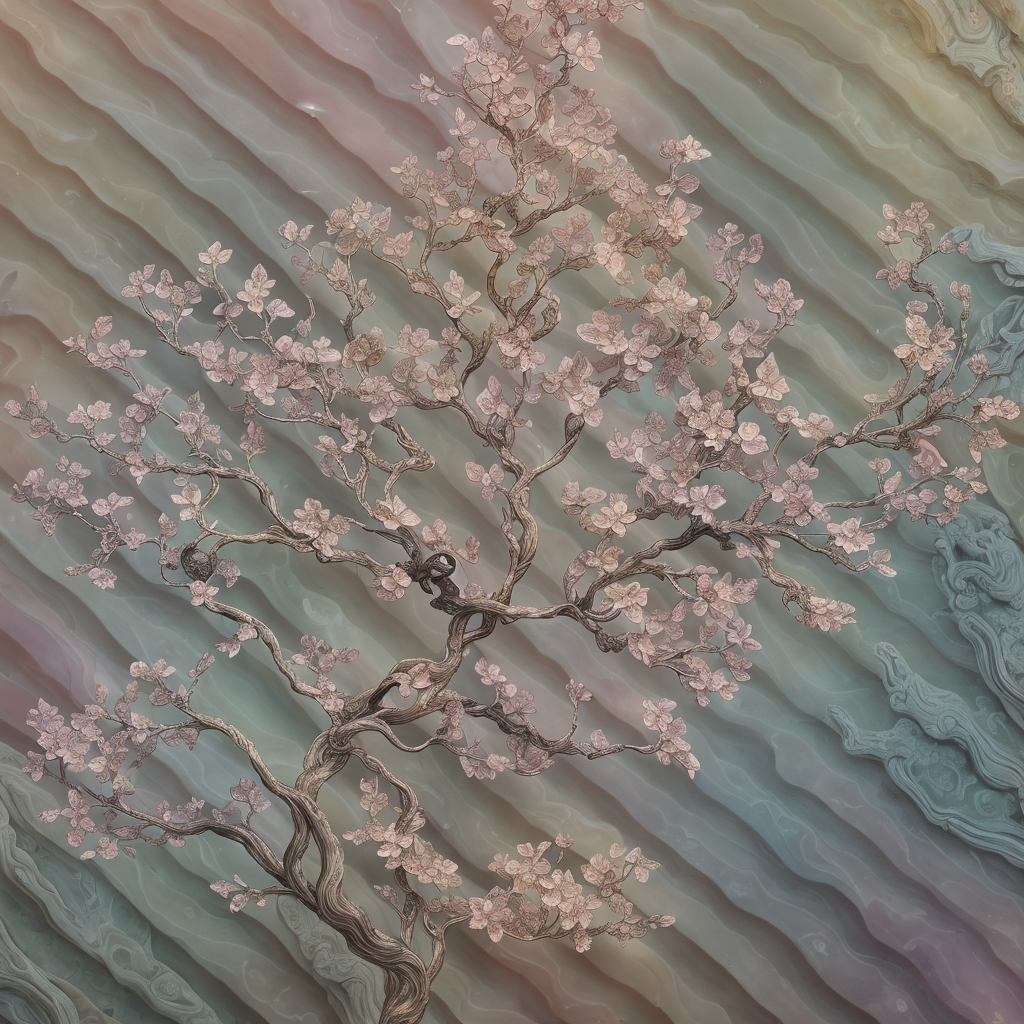
\includegraphics[width=0.5\textwidth]{../images/10.png}
	\caption{Сакура.}
\end{figure}

Далее я вычислю Фурье-образ изображения. 2D Фурье-образ - изображение, в котором каждый пиксель отвечает за определенную частоту в исходном изображении:

\begin{figure}[H]
	\centering
	\begin{minipage}{0.45\textwidth}
		\centering
		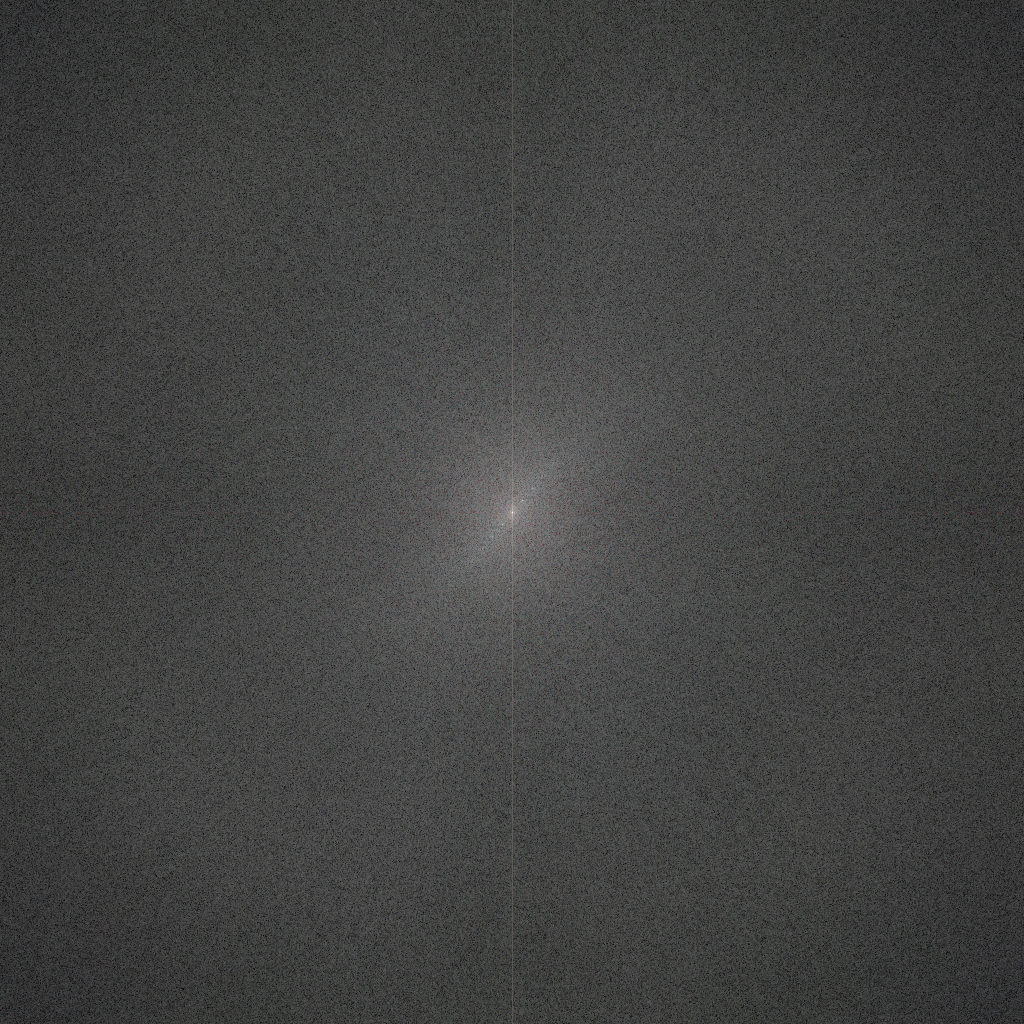
\includegraphics[width=\linewidth]{../images/logMagnitude.png}
		\caption{2D Фурье-образ.}
	\end{minipage}
	\hfill
	\begin{minipage}{0.45\textwidth}
		\centering
		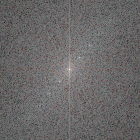
\includegraphics[width=\linewidth]{../images/logMagnitude2.png}
		\caption{2D Фурье-образ. Увеличенный.}
	\end{minipage}
\end{figure}


На изображении можно наблюдать яркие белые точки (пики). Избавлюсь от них с помощью фоторедактора - замажу черным цветом.


\begin{figure}[H]
	\centering
	\begin{minipage}{0.45\textwidth}
		\centering
		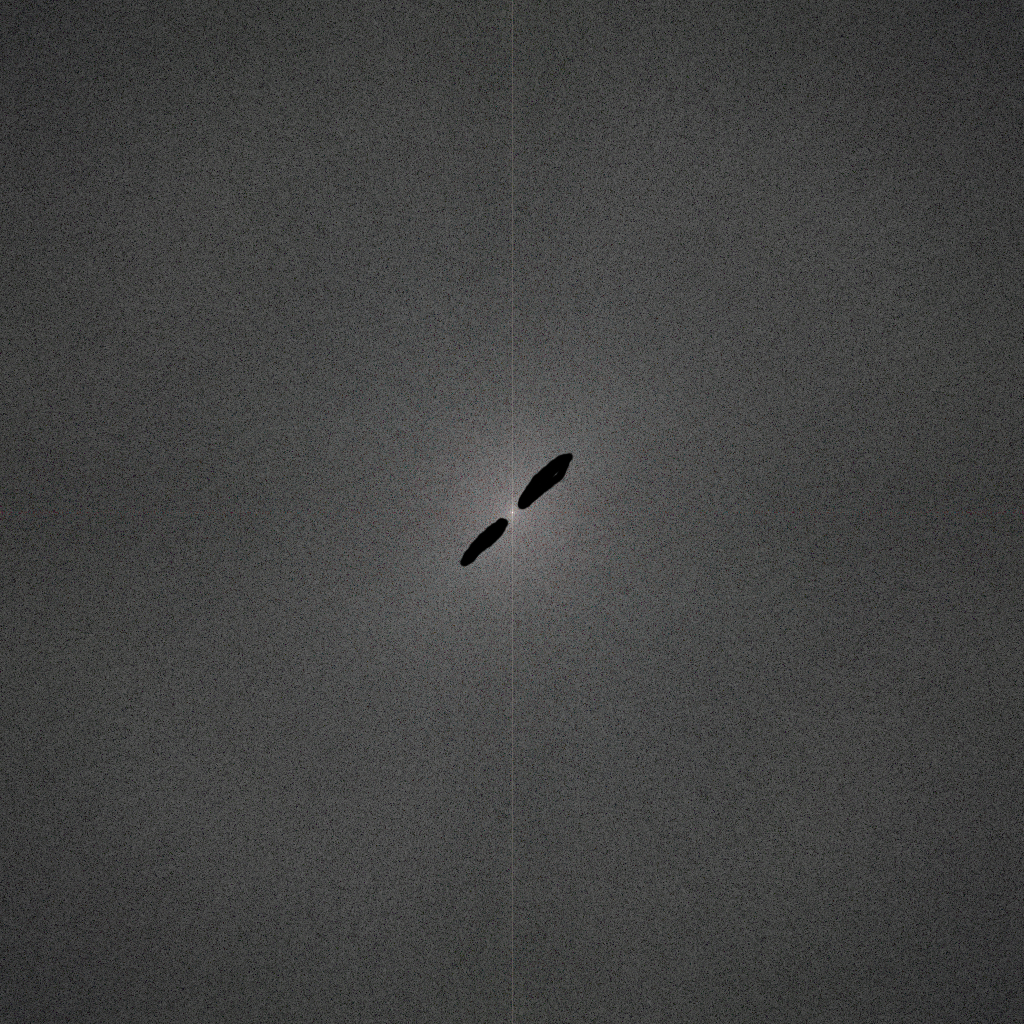
\includegraphics[width=\linewidth]{../images/rec5.jpg}
		\caption{Отфильтрованный 2D Фурье-образ.}
	\end{minipage}
	\hfill
	\begin{minipage}{0.45\textwidth}
		\centering
		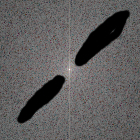
\includegraphics[width=\linewidth]{../images/rec52.jpg}
		\caption{Отфильтрованный 2D Фурье-образ. Увеличенный.}
	\end{minipage}
\end{figure}

Иными словами, замазав пики черным цветом я обнулила значения частот. Важно не обнулять центр спектра, так как он влияет на яркость его изображения.Когда я обнулила центральный пиксель, мое изображение стало заметно черным. Теперь попытаюсь восстановить изображение по полученному спектру. Для сравнения размещу исходную и фильтрованную картинки рядом.


\begin{figure}[H]
	\centering
	\begin{minipage}{0.45\textwidth}
		\centering
		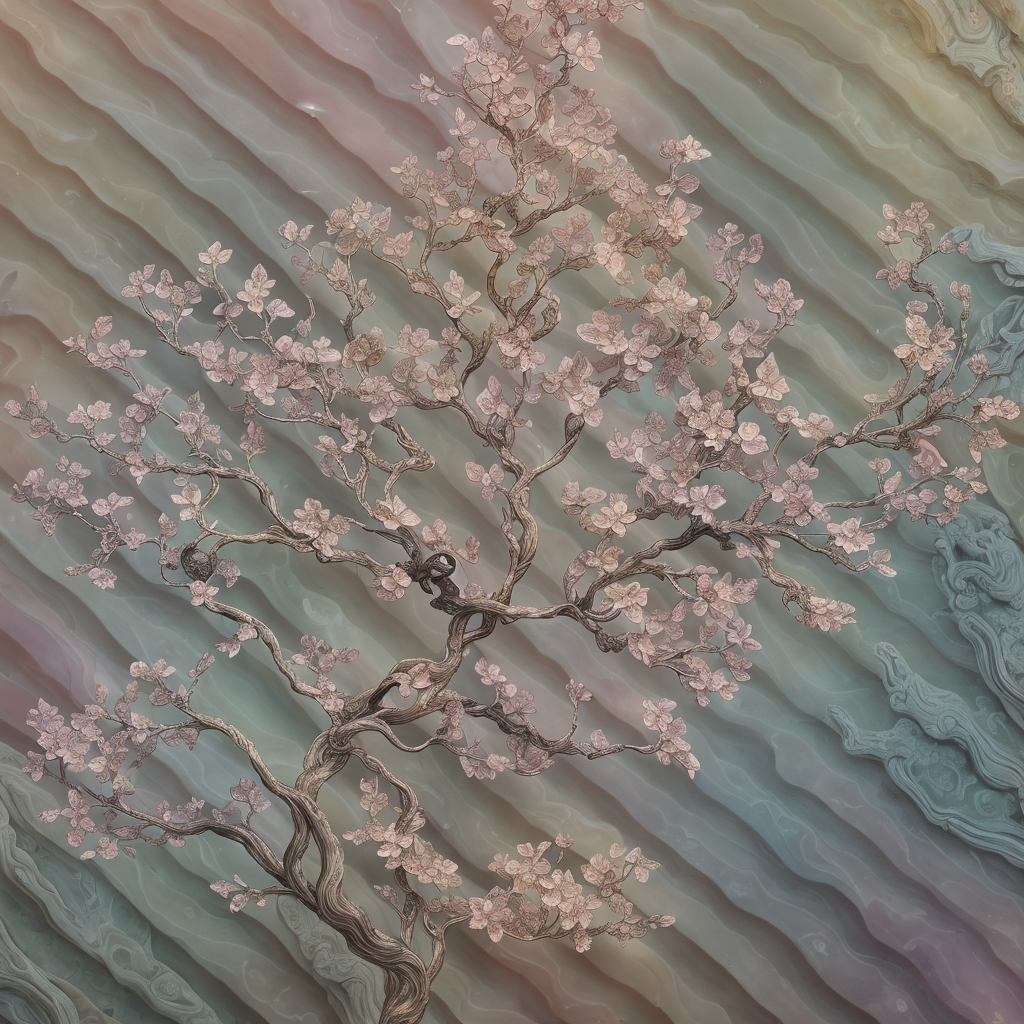
\includegraphics[width=\linewidth]{../images/10.png}
		\caption{Исходная сакура.}
	\end{minipage}
	\hfill
	\begin{minipage}{0.45\textwidth}
		\centering
		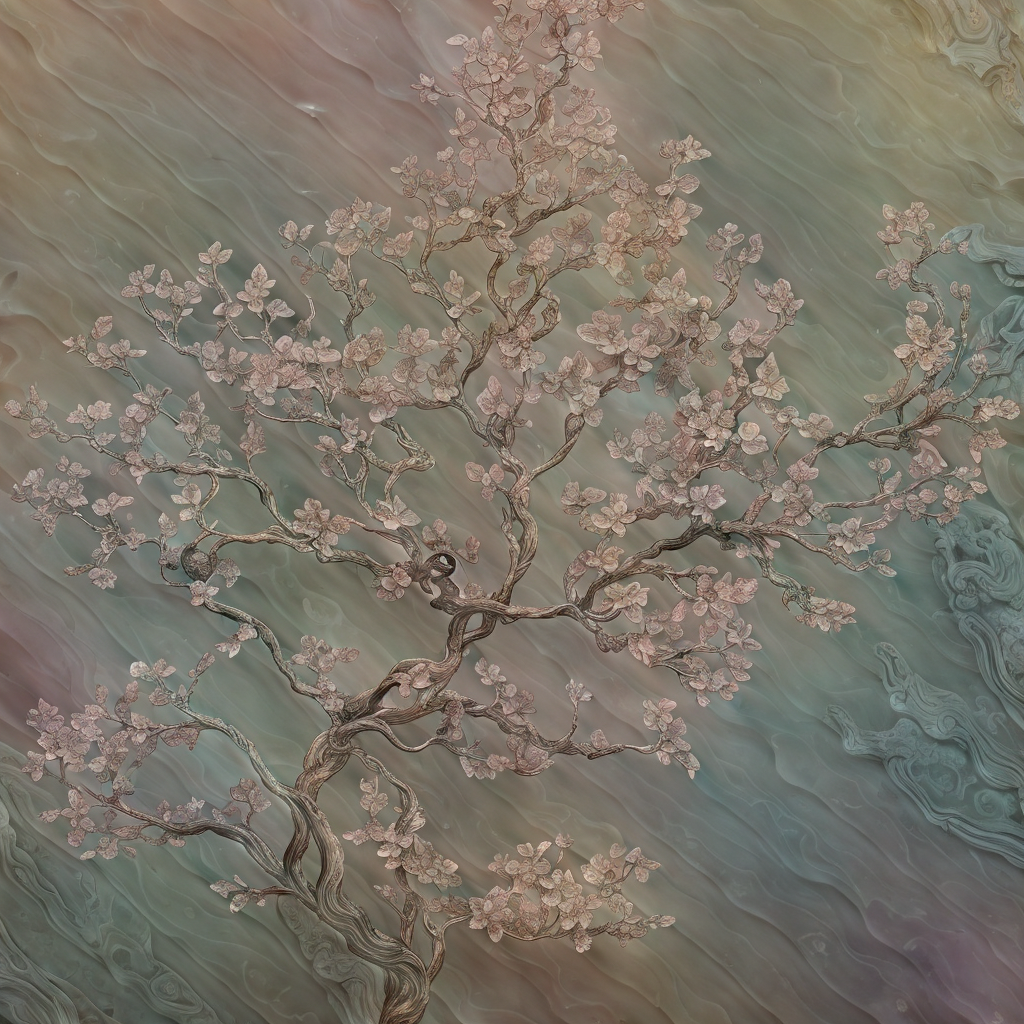
\includegraphics[width=\linewidth]{../images/final5.png}
		\caption{Отфильтрованная сакура.}
	\end{minipage}
\end{figure}

Заметно, что диагональные полосы с изображения ушли.


\subsection*{Вывод}

В этом задании я убрала периодические помехи с картинки с помощью Фурье-преобразования. Оказалось, что полосы на изображении сакуры соответствуют ярким точкам на Фурье-образе. Когда я убрала эти точки, полосы на картинке исчезли. При этом само изображение дерева осталось четким и не испортилось. 

\newpage

\section{Задание. Исследование свёртки.}

В этом задании я исследую применение различных ядер свертки для обработки изображений. Я выбрала pixel-art изображение и выполню следующие шаги:

Сначала я загружу изображение и преобразую его в черно-белое.

Затем я применю различные ядра свертки:

\begin{itemize}
	\item Гауссово размытие для трех нечётных значений $N \geq 3$:
	\[
	\sigma = \frac{N - 1}{6}, \quad A_{ij} = \exp\left(-\frac{(i - \frac{N+1}{2})^2 + (j - \frac{N+1}{2})^2}{2\sigma^2}\right)
	\]
	\[
	K_\sigma = \frac{A}{\sum_{i,j} A_{i,j}}
	\]
	
	\item Блочное размытие для тех же значений $N$:
	\[
	A_{ij} = 1, \quad K_\square = \frac{A}{\sum_{i,j} A_{i,j}}
	\]
	
	\item Увеличение резкости:
	\[
	K_* = \begin{bmatrix}
	0 & -1 & 0 \\
	-1 & 5 & -1 \\
	0 & -1 & 0
	\end{bmatrix}
	\]
	
	\item Выделение краёв:
	\[
	K_\nabla = \begin{bmatrix}
	-1 & -1 & -1 \\
	-1 & 8 & -1 \\
	-1 & -1 & -1
	\end{bmatrix}
	\]
	
	\item Произвольное ядро по своему выбору
\end{itemize}

Я выполню свёртку каждого ядра с исходным изображением и проанализирую результаты.

Затем я найду Фурье-образ исходного изображения и каждого ядра, заполнив пропуски нулями. Я поэлементно перемножу Фурье-образ изображения с Фурье-образами каждого ядра и выполню обратное преобразование Фурье.

В заключение я сравню изображения, полученные с помощью свёртки и Фурье-преобразования, а также отдельно сравню качество блочного и гауссовского размытия.
\[\]
\textbf{Ожидаемые результаты}
\begin{itemize}
	\item Исходное черно-белое изображение
	\item Спектр исходного изображения
	\item Фильтрованные изображения разными ядрами
	\item Спектры всех ядер свертки
	\item Сравнение результатов пространственной и частотной фильтрации
	\item Анализ полученных результатов и выводы
\end{itemize}

\hrule
\[\]
Приступлю к заданию. Выберу пиксельное изображение капибары и отрисую логарифм модуля Фурье-образа картинки.

\begin{figure}[H]
	\centering
	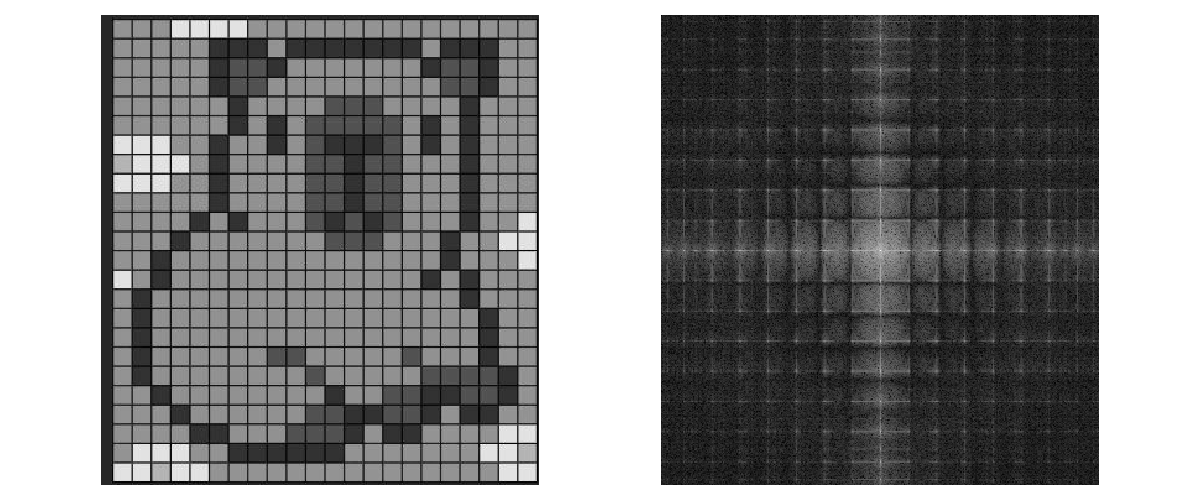
\includegraphics[width=1\textwidth]{../images/cap.png}
	\caption{Изображение и ее логарифм модуля Фурье-образа.}
\end{figure}


\subsection{Гауссово размытие}

Гауссово размытие подавляет шум и размывает изображение. Посмотрим на изображения после свертки и фильтрации, а также рассмотрим их спектры соответственно.

\textbf{\(N = 5\) }:

\begin{figure}[H]
	\centering
	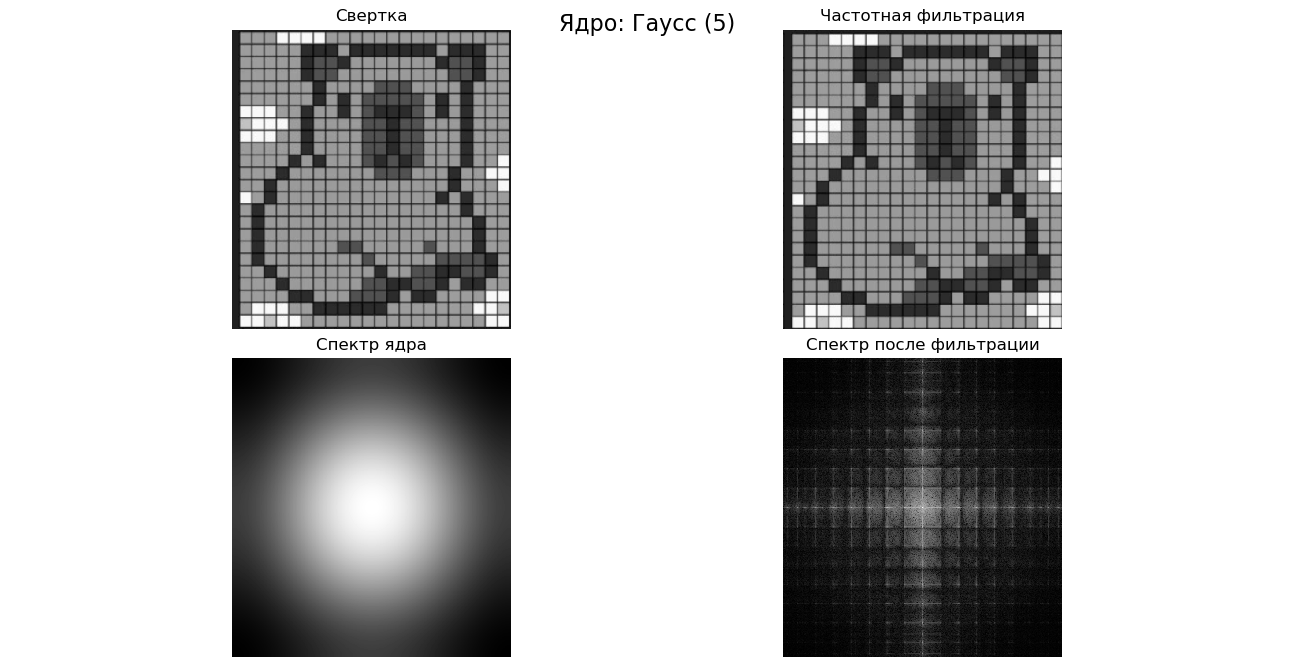
\includegraphics[width=1\textwidth]{../images/gaus5.png}
	\caption{Гауссово размытие. \(N = 5\)}
\end{figure}

\textbf{\(N = 7\) }:

\begin{figure}[H]
	\centering
	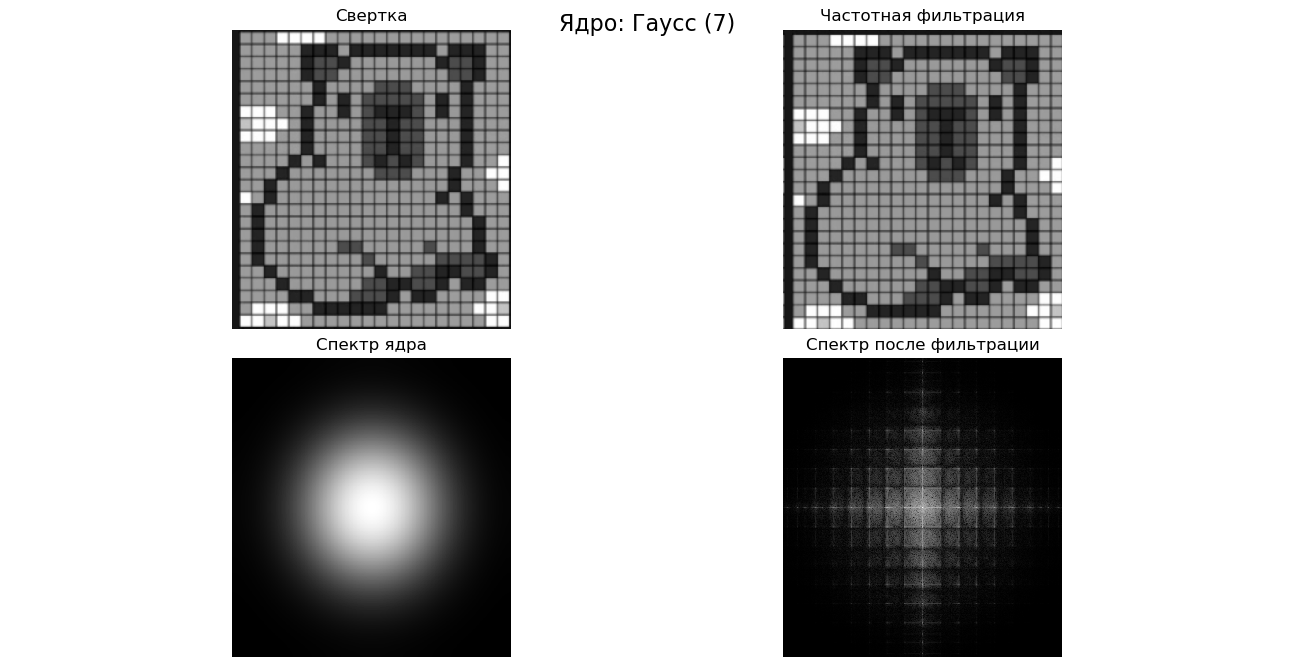
\includegraphics[width=1\textwidth]{../images/gaus7.png}
	\caption{Гауссово размытие. \(N = 7\)}
\end{figure}

\textbf{\(N = 21\) }:

\begin{figure}[H]
	\centering
	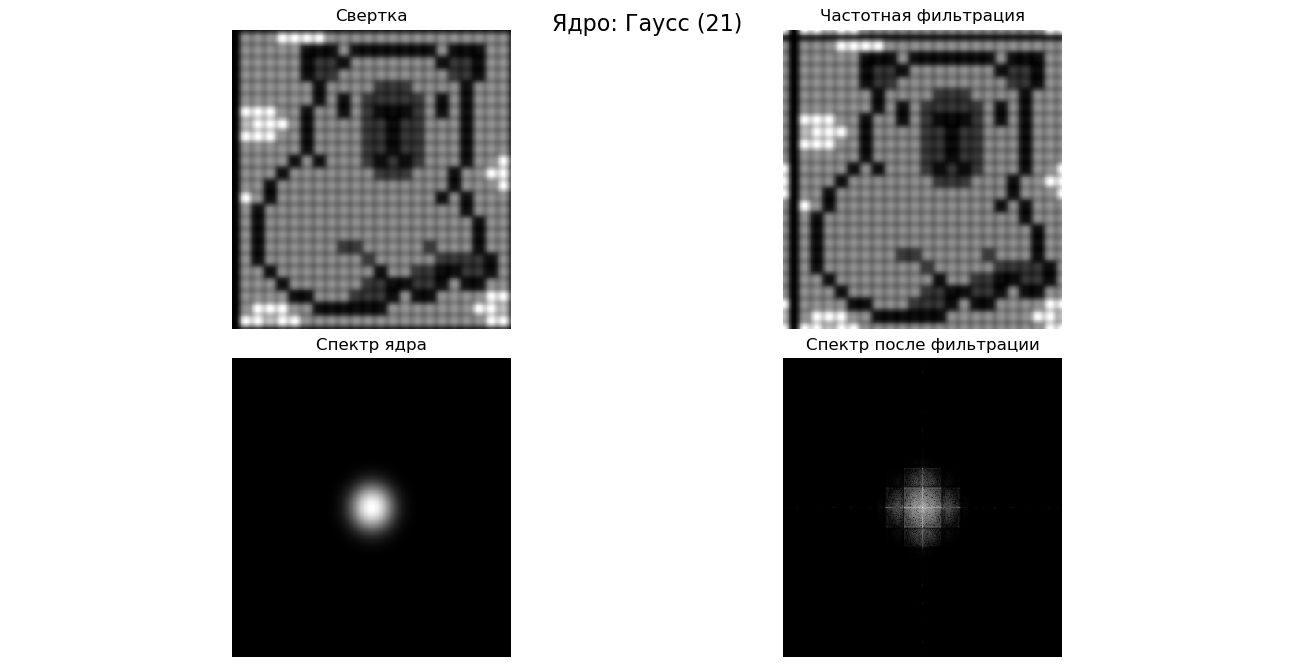
\includegraphics[width=1\textwidth]{../images/gaus11.png}
	\caption{Гауссово размытие. \(N = 21\)}
\end{figure}

\textbf{Итог: } При  увеличении параметра \(N\) увеличивается степень рамытия. Однако важно понимать, что если мы имеем дело с детализированным изображением, мелкие детали затеряются.  

\subsection{Блочное размытие}

Попробую размыть изображения с помощью блочного фильтра.

\textbf{\(N = 5\) }:

\begin{figure}[H]
	\centering
	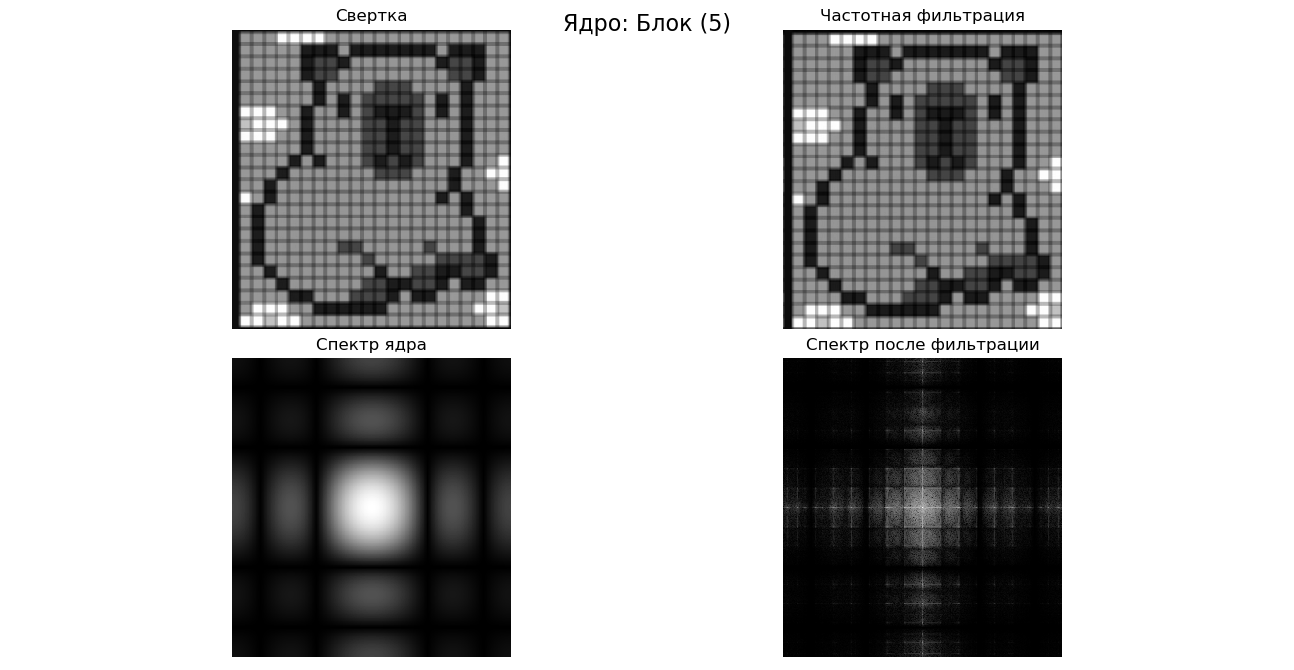
\includegraphics[width=1\textwidth]{../images/blok5.png}
	\caption{Блочное размытие. \(N = 5\)}
\end{figure}

\textbf{\(N = 7\) }:

\begin{figure}[H]
	\centering
	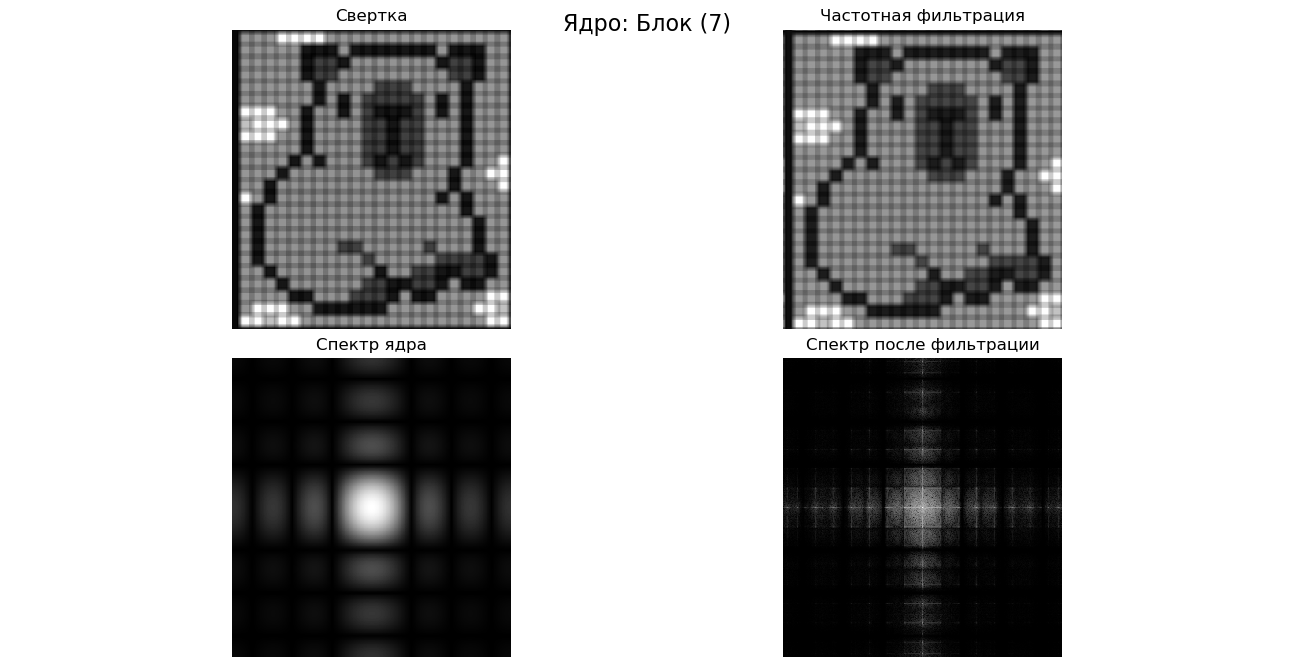
\includegraphics[width=1\textwidth]{../images/blok7.png}
	\caption{Блочное размытие. \(N = 7\)}
\end{figure}

\textbf{\(N = 11\) }:

\begin{figure}[H]
	\centering
	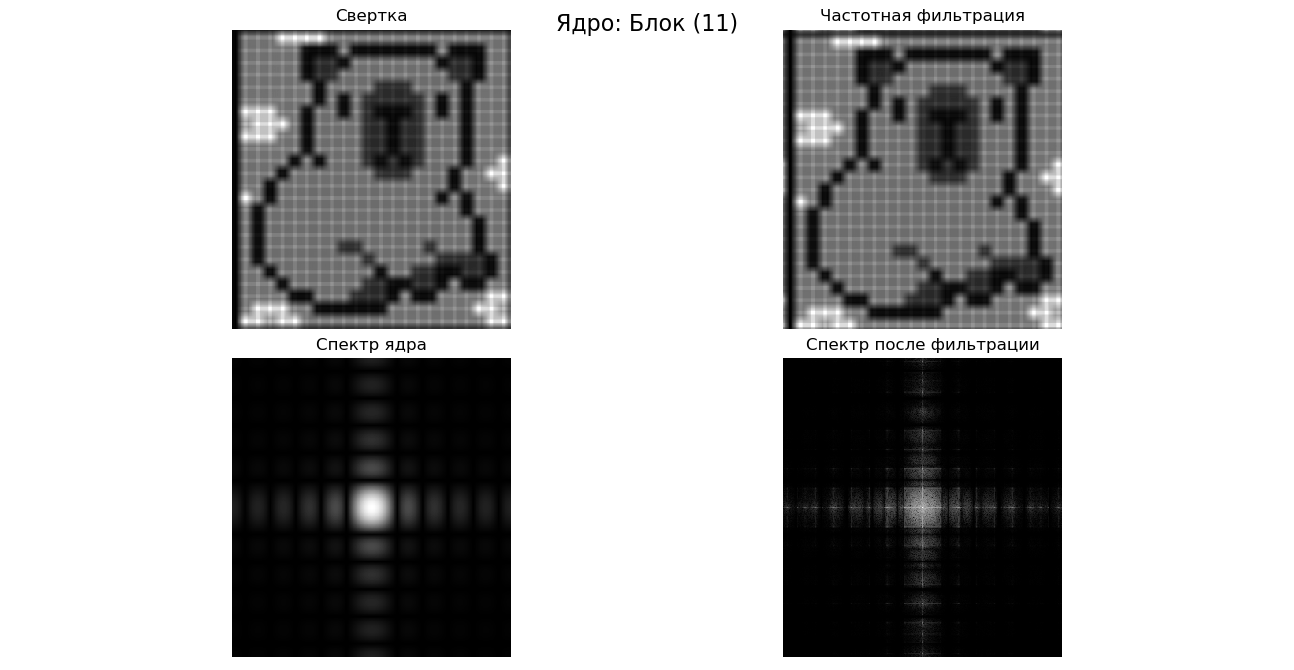
\includegraphics[width=1\textwidth]{../images/blok11.png}
	\caption{Блочное размытие. \(N = 21\)}
\end{figure}

\textbf{Итог: } Блочное размытие может создавать артефакты в виде "блочности" на границах объектов, что особенно заметно при больших значениях \(N\). Этот метод прост в реализации, но менее качественен по сравнению с гауссовым размытием.

\subsection{Увеличение резкости}

Фильтр увеличения резкости эффективно подчеркивает детали изображения и усиливает контраст на границах объектов. 
\begin{figure}[H]
	\centering
	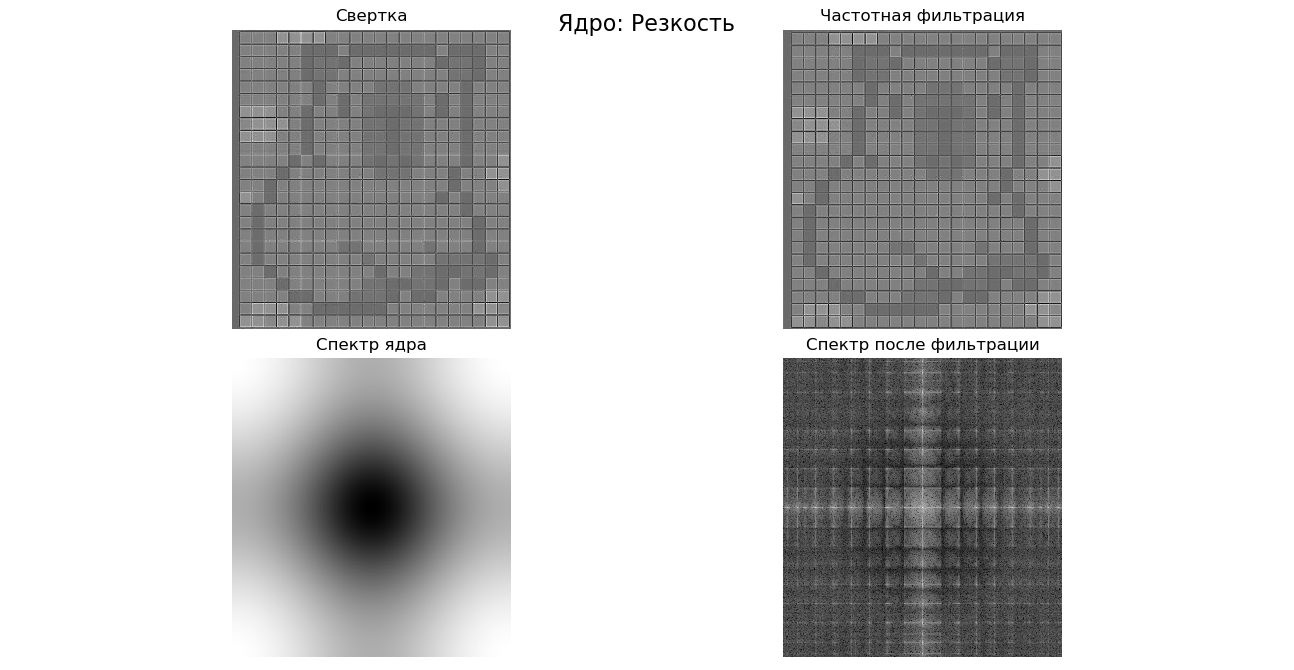
\includegraphics[width=1\textwidth]{../images/rezko.png}
	\caption{Увеличение резкости.}
\end{figure}

\textbf{Итог: } Увеличение резкости полезно для улучшения качества изображений, потерявших четкость при съемке или обработке.

\subsection{Выделение краев}

С помощью этого ядра попробую извлечь контуры у изображения.

\begin{figure}[H]
	\centering
	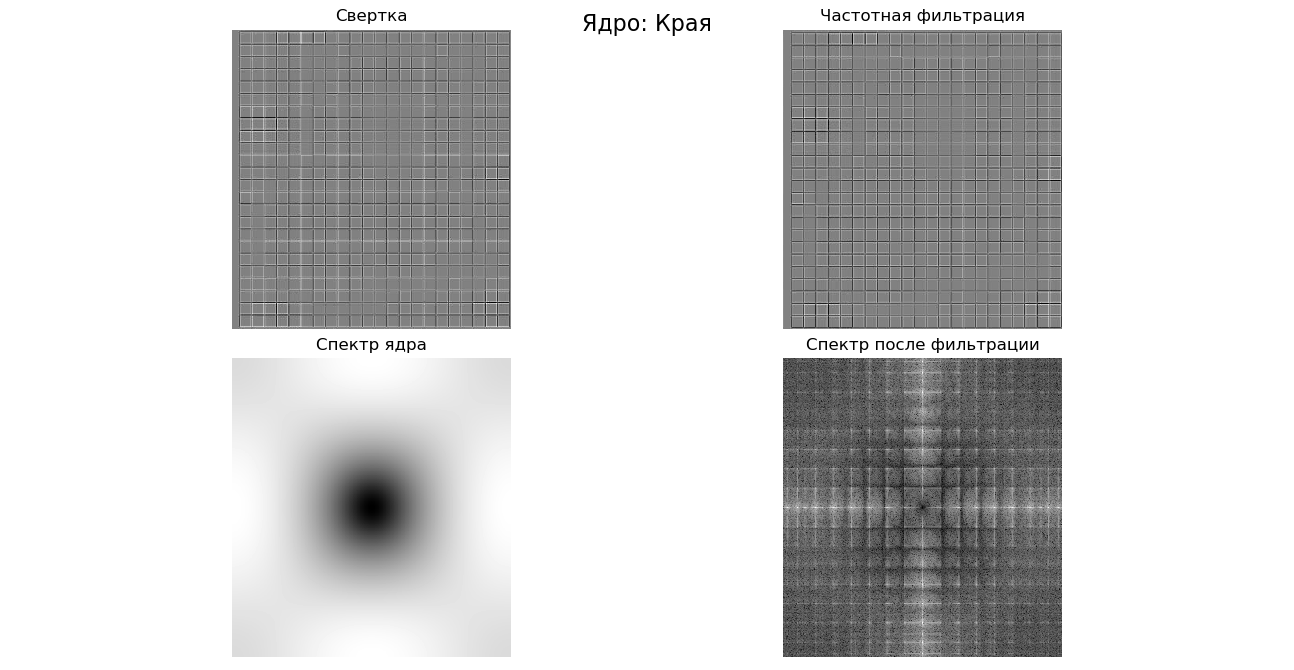
\includegraphics[width=1\textwidth]{../images/kraya.png}
	\caption{Выделение краев.}
\end{figure}

\textbf{Итог: } Появились слабозаметные очертания картинки. Однако шума на изображении стало больше.

\subsection{Алгоритм Canny}

Так как в предыдущем пункте не особо удалось увидеть края у изображения, попытаюсь это сделать по алгоритму Кэнни. Вот так он работает:

\begin{itemize}
	\item Применяем гауссово размытие
	\item Вычисляем градиенты (операторы Собеля по X и Y):
	\[
	G_x = \begin{bmatrix} -1 & 0 & 1 \\ -2 & 0 & 2 \\ -1 & 0 & 1 \end{bmatrix}, \quad
	G_y = \begin{bmatrix} -1 & -2 & -1 \\ 0 & 0 & 0 \\ 1 & 2 & 1 \end{bmatrix}
	\]
	\item Далее утончаем границы - оставляем только самые четкие линии
\end{itemize}

Посмотрим на результат!

\begin{figure}[H]
	\centering
	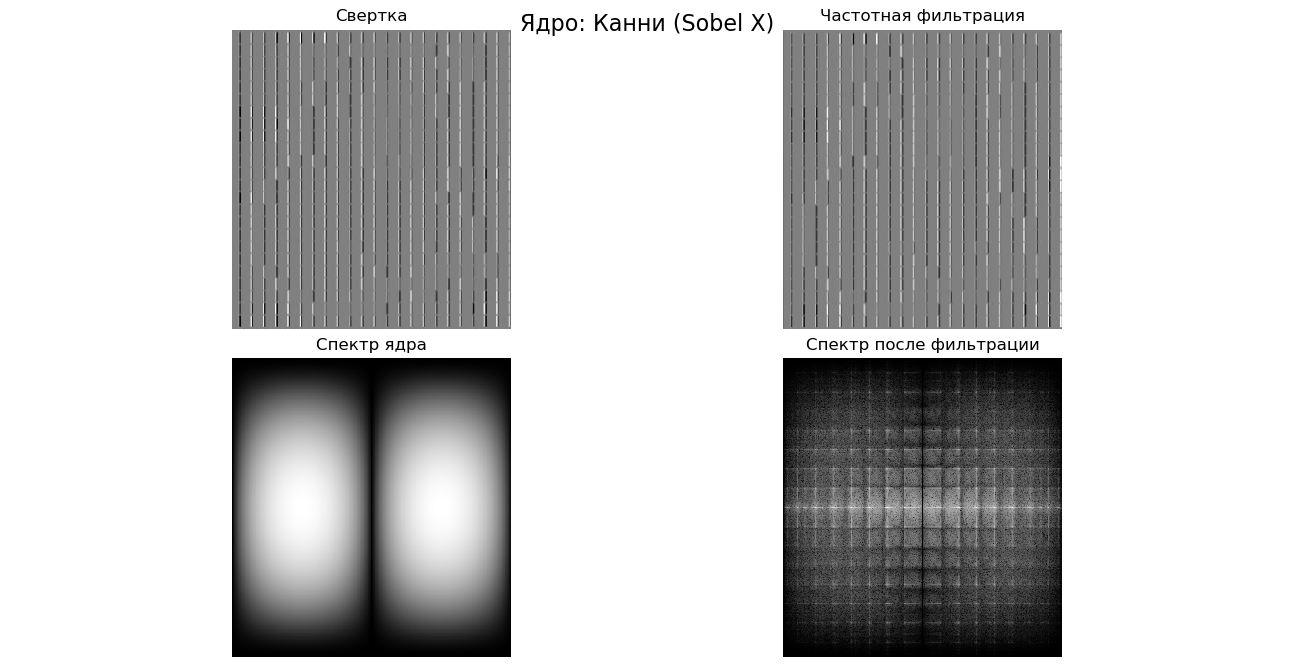
\includegraphics[width=1\textwidth]{../images/X.png}
	\caption{Алгоритм Канни \(X\).}
\end{figure}

\begin{figure}[H]
	\centering
	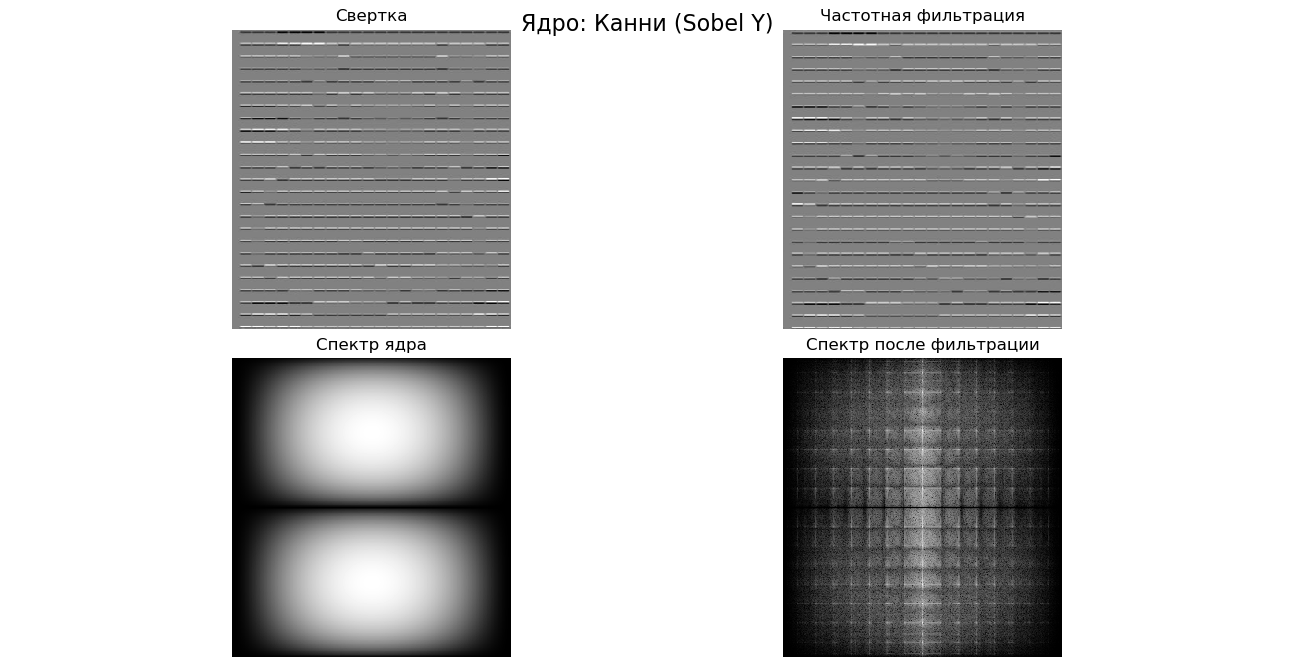
\includegraphics[width=1\textwidth]{../images/Y.png}
	\caption{Алгоритм Канни \(Y\).}
\end{figure}

\textbf{Итог: } Алгоритм Канни отлично справился с обнаружением границ! Оператор Собеля по X хорошо выделил вертикальные границы, а оператор по Y - горизонтальные. Этот метод оказался эффективнее фильтра выделения краёв - границы получились более чёткими и непрерывными, без лишнего шума.

\subsection{Сравнение качество блочного и гауссовского размытий.}

Сравнивая два типа размытия, я пришла к следующим выводам:

\begin{itemize}
	\item Гауссово размытие дает более естественное и плавное размытие изображения, в то время как блочное размытие создает заметные артефакты и "блочность" на границах объектов.
	
	\item Оба метода эффективно устраняют мелкие детали и шумы, но гауссово размытие лучше сохраняет общие очертания объектов.
	
	\item Изображения, обработанные гауссовым фильтром, выглядят более профессионально.

\end{itemize}


\subsection{Вывод}

В ходе выполнения задания я исследовала применение различных ядер свертки для обработки изображений. Мне удалось на практике изучить, как разные фильтры влияют на изображение и какие эффекты они создают. Я убедилась, что гауссово размытие дает более качественный результат по сравнению с блочным - оно создает плавное естественное размытие без артефактов. Также я обнаружила, что алгоритм Кэнни значительно эффективнее простого фильтра выделения краёв, так как он лучше справляется с обнаружением границ и меньше подвержен шуму. Фильтр увеличения резкости отлично подходит для улучшения чёткости изображений. В целом, задание помогло мне понять, как выбирать подходящие фильтры для разных задач обработки изображений и как они работают на практике.

\newpage

\section{Вывод}
В ходе работы я освоила методы обработки изображений с использованием преобразования Фурье и операций свертки. Научилась фильтровать периодические шумы через частотную область и применять различные ядра свертки для размытия, повышения резкости и выделения границ.

\newpage

\section{Приложение}

\begin{lstlisting}[language=python, caption=Ядра для задания 2]
kernels = {
	"Gaus (5)": create_gaussian_kernel(5),
	"Gaus (7)": create_gaussian_kernel(7),
	"Gaus (21)": create_gaussian_kernel(21),
	"Gaus (5)": create_box_kernel(5),
	"Gaus (7)": create_box_kernel(7),
	"Gaus (11)": create_box_kernel(11),
	"Rezkoct": np.array([[0, -1, 0], [-1, 5, -1], [0, -1, 0]]),
	"Kraya": np.array([[-1, -1, -1], [-1, 8, -1], [-1, -1, -1]]),
	"Canny (Sobel X)": np.array([[-1, 0, 1], [-2, 0, 2], [-1, 0, 1]]),
	"Canny (Sobel Y)": np.array([[-1, -2, -1], [0, 0, 0], [1, 2, 1]])
}
\end{lstlisting}


\end{document}

	
	